%% ============================================================
%% Revision Notes (2026-03-29, Yuyang):
%% 1. Core Principle: Already concise, kept as-is.
%% 2. Typology of Guardrail Mechanisms: Shortened each type description,
%%    especially Model-Based (compressed historical toxicity detection work).
%% 3. Applications: Split combined Safety+Privacy and Fairness+Factuality
%%    paragraphs into four separate \paragraph entries, one per domain.
%% 4. Discussion: Removed from this file. Shortened version moved to
%%    sections/11-challenges_directions.tex with red source marker.
%% ============================================================

\subsection{Guardrails}
\label{sec:guardrails}

\begin{figure}[htbp]
\centering
% Width uses \textwidth; height auto-scales with !
\resizebox{\textwidth}{!}{%
\begin{tikzpicture}
% --- 1. Define leaf nodes (papers, citations added) ---
\node[leaf] (safety_papers) {
NeMo Guardrails~\citep{Rebedea2023NeMoGA}, LlamaFirewall~\citep{Chennabasappa2025LlamaFirewallAO}, Wildflare GuardRail~\citep{Han2025BridgingTS}, SoK~\citep{Wang2025SoKEJ}, Llama Guard~\citep{Inan2023LlamaGL, Chi2024LlamaG3}, Constitutional Classifiers~\citep{Sharma2025ConstitutionalCD}, WildGuard~\citep{Han2024WildGuardOO}, Granite Guardian~\citep{Padhi2024GraniteG}, ShieldGemma~\citep{Zeng2024ShieldGemmaGA, Zeng2025ShieldGemma2R}, PolyGuard~\citep{Kumar2025PolyGuardAM}, X-Guard~\citep{Upadhayay2025XGuardMG}, AEGIS~\citep{Ghosh2024AEGISOA}, SafeRoute~\citep{Lee2025SafeRouteAM}, LLM-as-a-Judge~\citep{Zheng2023JudgingLW}, GuardReasoner~\citep{Liu2025GuardReasonerTR}, R$^2$-Guard~\citep{Kang2024R2GuardRR}, RSafe~\citep{Zheng2025RSafeIP}, Palisade~\citep{Kokkula2024PalisadeP}, Rebuff~\citep{Rebuff2023}, Azure Prompt Shield~\citep{azure2025promptshields}, Prompt Guard~\citep{meta2025promptguard}, Zou et al.~\citep{Zou2023UniversalAT}, ArtPrompt~\citep{Jiang2024ArtPromptAA}, Hackett et al.~\citep{hackett2025bypassing}, POSTERIAL~\citep{Jiang2023POSTERIA}.
};
\node[leaf, below=0.3cm of safety_papers] (privacy_papers) {
Llama Guard~\citep{Chi2024LlamaG3}, Azure Prompt Shield~\citep{azure2025promptshields}.
};
\node[leaf, below=0.3cm of privacy_papers] (fairness_papers) {
Davidson et al.~\citep{Davidson2017AutomatedHS}, Borkan et al.~\citep{Borkan2019NuancedMF}, HateXplain~\citep{Mathew2020HateXplainAB}, ToxiGen~\citep{Hartvigsen2022ToxiGenAL}, Perspective API~\citep{Lees2022ANG}.
};
\node[leaf, below=0.3cm of fairness_papers] (factuality_papers) {
(Limited recent guardrail-specific research; see §\ref{sec:guardrails}).
};
% --- 2. Define main sub-nodes (Trustworthiness dimensions) ---
% Positioned to the left of corresponding leaf nodes
\node[sub, left=0.5cm of safety_papers] (safety) {Safety};
\node[sub, left=0.5cm of privacy_papers] (privacy) {Privacy};
\node[sub, left=0.5cm of fairness_papers] (fairness) {Fairness};
\node[sub, left=0.5cm of factuality_papers] (factuality) {Factuality \& Faithfulness};
% --- 3. Define root node ---
% Use the calc library to vertically center the root node relative to the sub-nodes
\node[main, left=2.5cm of {$(safety.west)!0.5!(factuality.west)$}] (guardrails) {Guardrails (§\ref{sec:guardrails})};
% --- 4. Draw connection lines ---
% a. Draw a main trunk from the root node to a branching point
\coordinate (fork) at ($(guardrails.east)+(1.25cm,0)$);
\draw[line] (guardrails.east) -- (fork);
% b. Connect from main branching point to each sub-node
\draw[line] (fork) |- (safety.west);
\draw[line] (fork) |- (privacy.west);
\draw[line] (fork) |- (fairness.west);
\draw[line] (fork) |- (factuality.west);
% c. Connect main sub-nodes directly to leaf nodes
\draw[line] (safety.east) -- (safety_papers.west);
\draw[line] (privacy.east) -- (privacy_papers.west);
\draw[line] (fairness.east) -- (fairness_papers.west);
\draw[line] (factuality.east) -- (factuality_papers.west);
\end{tikzpicture}%
}
\caption{A taxonomy of Guardrails for enhancing LLM trustworthiness.}
\label{fig:guardrails_taxonomy}
\end{figure}

\subsubsection{Core Principle: Modular and External Control}

Guardrails provide a modular and external mechanism for controlling LLM behavior, operating as independent components that monitor and filter inputs or outputs without modifying the model's parameters. Unlike training-time interventions, guardrails function post-deployment, treating the LLM as a black-box system. This external positioning enables rapid deployment and updates, allowing systems to quickly adapt to evolving safety requirements and emerging threats. Their modular design supports flexible integration into existing pipelines, where multiple guardrails can be layered or combined to target specific risks. As external controls, guardrails ensure trustworthy outputs by intercepting potentially harmful content before it reaches the user or by regenerating outputs when violations are detected. While this  principle draws conceptually from traditional content moderation systems, it is now tailored to the dynamic and interactive nature of LLMs, emphasizing flexibility and minimal interference with the model's core functionality.

\begin{figure*}[htbp]
  \centering
  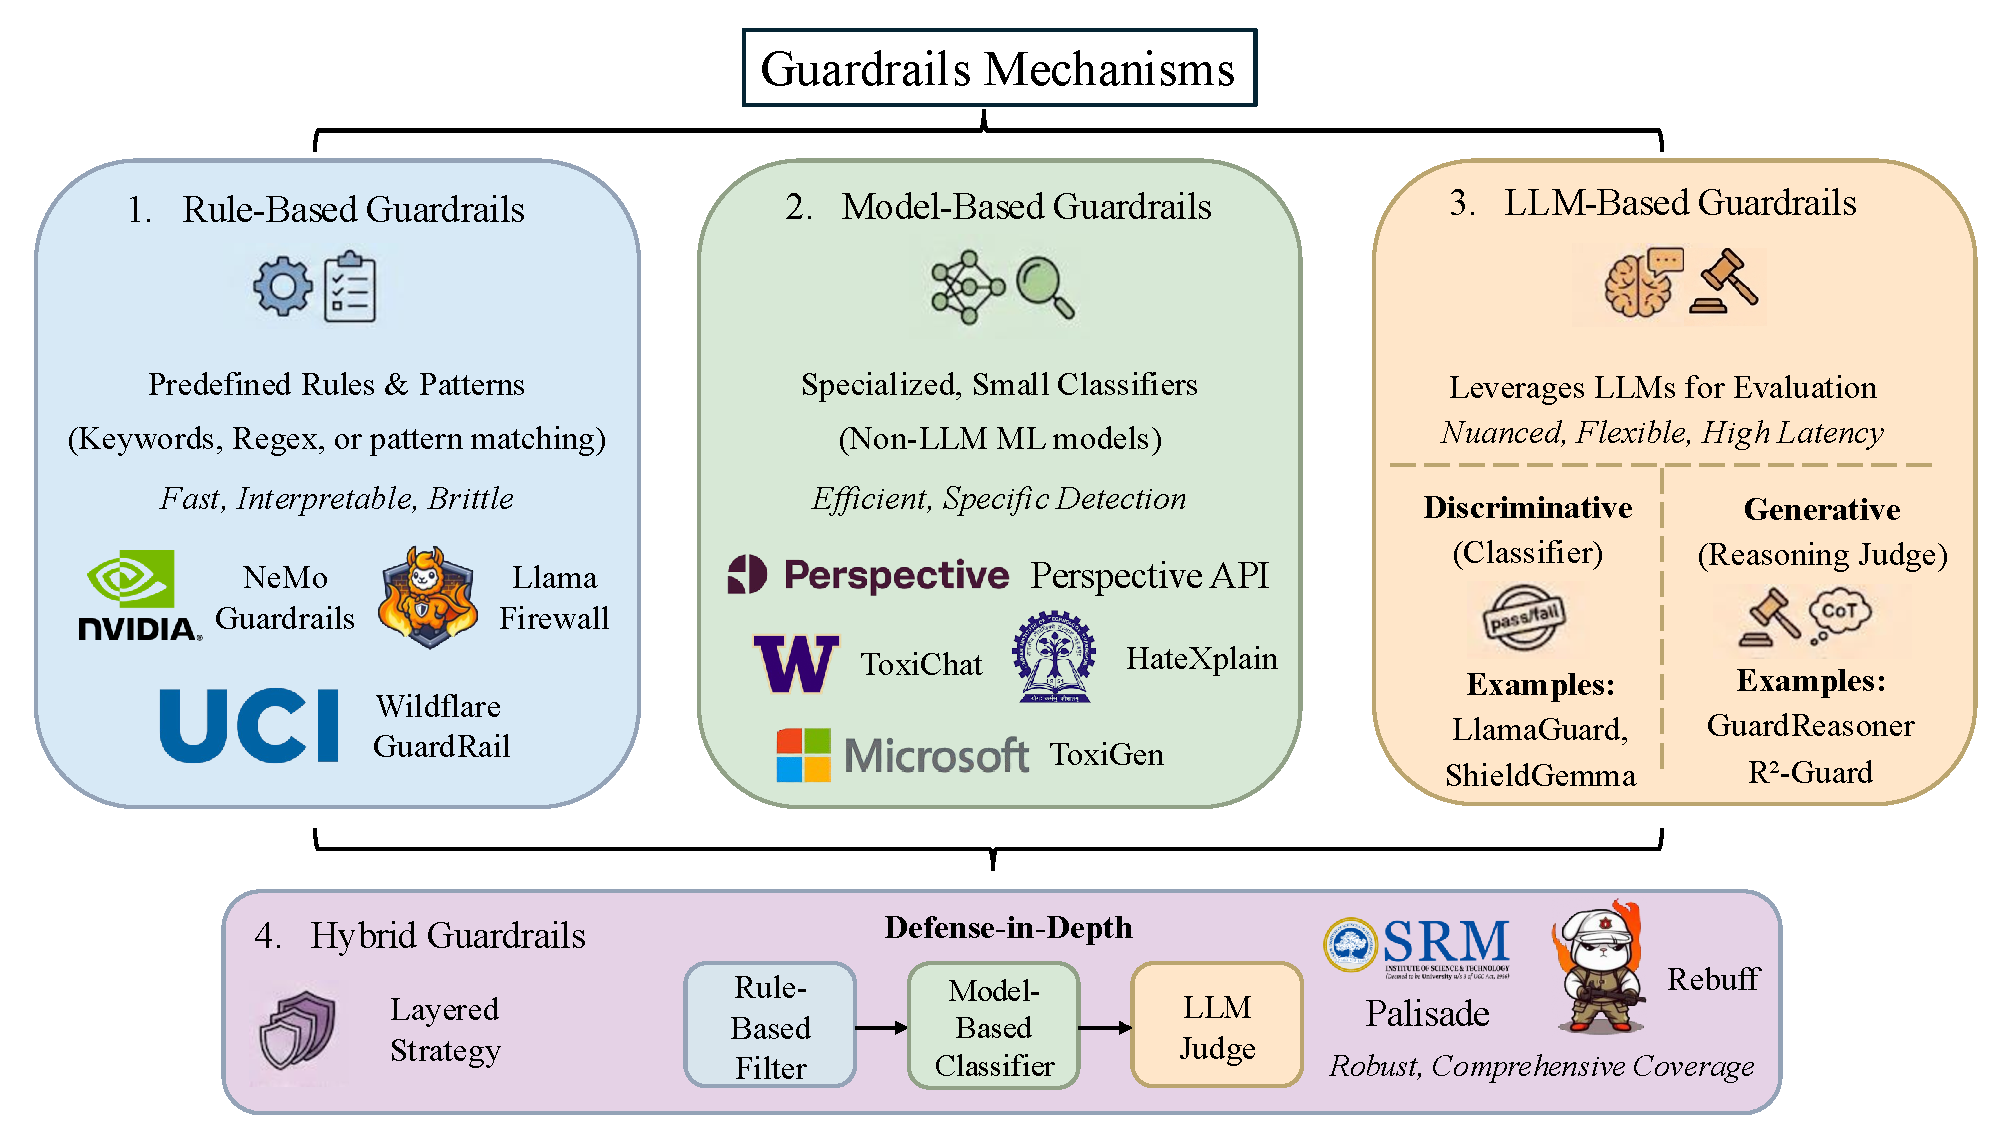
\includegraphics[width=0.9\linewidth]{figures/method/guardrails_new.pdf}
  \caption{A typology of guardrail mechanisms for LLM trustworthiness. The four categories---Rule-Based, Model-Based, LLM-Based (discriminative and generative), and Hybrid---are distinguished by their underlying detection approach, with representative systems shown for each. Hybrid guardrails combine multiple mechanism types in a layered ``defense-in-depth'' strategy for comprehensive coverage.}
  \label{fig:method_guardrails}
\end{figure*}


\subsubsection{A Typology of Guardrail Mechanisms}

Guardrail mechanisms can be classified according to their underlying approach, spanning from simple deterministic techniques to advanced LLM-driven systems.

\paragraph{Rule-Based Guardrails}

Rule-based guardrails rely on predefined rules, such as keyword lists, regular expressions, or pattern matching, to detect and filter prohibited content. For example, NeMo Guardrails~\citep{Rebedea2023NeMoGA} introduces programmable rails for dialog flow, topic blocking, and tool use; LlamaFirewall~\citep{Chennabasappa2025LlamaFirewallAO} incorporates customizable scanners including regex-based code filters for agentic workflows; and Wildflare GuardRail~\citep{Han2025BridgingTS} integrates modular rule-based wrappers as part of a multi-stage pipeline. While transparent and low-latency, these systems are brittle against novel adversarial strategies specific to LLMs, such as prompt injection and jailbreak attacks~\citep{Wang2025SoKEJ}.

\paragraph{Model-Based Guardrails}

Model-based guardrails employ smaller, specialized classifiers---typically non-LLM models such as neural networks or fine-tuned smaller transformers---for nuanced detection of safety violations. Early work focused on hate speech and toxicity detection, addressing challenges such as distinguishing hate speech from offensive content~\citep{Davidson2017AutomatedHS}, fairness-oriented evaluation for toxicity detectors~\citep{Borkan2019NuancedMF}, and adversarially generated datasets for implicit toxicity~\citep{Hartvigsen2022ToxiGenAL}. These insights informed practical deployments such as the Perspective API~\citep{Lees2022ANG}, which detects toxicity across languages, and explainable models like HateXplain~\citep{Mathew2020HateXplainAB} that provide human rationales alongside labels.

\paragraph{LLM-Based Guardrails}

LLM-based guardrails employ another large language model to evaluate and filter generated content, capturing nuance, abstraction, and intent that smaller classifiers often miss. Discriminative guardrails use LLMs as safety classifiers: Llama Guard~\citep{Inan2023LlamaGL, Chi2024LlamaG3} detects unsafe multimodal content categories, while Constitutional Classifiers~\citep{Sharma2025ConstitutionalCD}, WildGuard~\citep{Han2024WildGuardOO}, Granite Guardian~\citep{Padhi2024GraniteG}, and ShieldGemma~\citep{Zeng2024ShieldGemmaGA, Zeng2025ShieldGemma2R} provide fine-tuned drop-in safety classifiers. Recent work has expanded to multilingual coverage with PolyGuard~\citep{Kumar2025PolyGuardAM} and X-Guard~\citep{Upadhayay2025XGuardMG}, while ensemble approaches like AEGIS~\citep{Ghosh2024AEGISOA} and adaptive routing via SafeRoute~\citep{Lee2025SafeRouteAM} reflect a shift toward scalable, real-time solutions. Generative (reasoning) guardrails employ an LLM as a deliberative judge that critiques and justifies another model's output. Building on the LLM-as-a-judge paradigm~\citep{Zheng2023JudgingLW}, recent methods incorporate explicit reasoning chains before producing verdicts, such as GuardReasoner~\citep{Liu2025GuardReasonerTR}, R$^2$-Guard~\citep{Kang2024R2GuardRR} with knowledge-enhanced logical reasoning, GuardAdvisor~\citep{huang2026guardian} with a soft-gating pipeline, and RSafe~\citep{Zheng2025RSafeIP} with adaptive guided safety reasoning.

\paragraph{Hybrid Guardrails}

Hybrid guardrails combine multiple mechanisms for comprehensive coverage through a ``defense-in-depth'' strategy. For example, Palisade~\citep{Kokkula2024PalisadeP} proposes a three-layer pipeline combining a rule-based filter, an ML classifier, and a companion-LLM check, while Rebuff~\citep{Rebuff2023} integrates heuristics, canary tokens, a database of known attacks, and an LLM-based check.

\subsubsection{Applications}

\paragraph{Safety}

Guardrails are predominantly applied in safety, where they serve as critical defenses against emerging threats inherent to LLMs. On the input side, guardrails detect and block attacks such as jailbreaks that aim to bypass alignment constraints~\citep{Zou2023UniversalAT, Jiang2024ArtPromptAA} and prompt injections where adversaries embed malicious instructions to hijack model outputs~\citep{hackett2025bypassing, Jiang2023POSTERIA}. Systems like Azure Prompt Shield~\citep{azure2025promptshields} and Prompt Guard~\citep{meta2025promptguard} employ adversarial-input detectors to identify injection attempts and block unsafe prompts. On the output side, guardrails evaluate and filter model generations before delivery to end users, with systems like Llama Guard~\citep{Chi2024LlamaG3} enforcing a taxonomy of unsafe categories---including violent crimes, sex crimes and child exploitation, defamation, hate speech, self-harm, and election misinformation---by classifying outputs and blocking or regenerating unsafe completions.

\paragraph{Privacy}

In the privacy domain, guardrails protect against the disclosure of personal or sensitive information. Output-side guardrails can classify and block generations that contain personally identifiable information, confidential data, or intellectual property violations. Systems such as Llama Guard~\citep{Chi2024LlamaG3} include disclosure of sensitive information as an explicit unsafe category, while Azure Prompt Shield~\citep{azure2025promptshields} detects attempts to exfiltrate private data through prompt injection. However, guardrail-specific research for privacy remains limited compared to safety, and most privacy protections are currently bundled within broader safety taxonomies rather than addressed by dedicated guardrail mechanisms.

\paragraph{Fairness}

Guardrails for fairness have historical roots in pre-LLM content moderation, where classifiers were designed to detect and reduce bias in generated content~\citep{Borkan2019NuancedMF, Mathew2020HateXplainAB}. Toxicity and hate speech detectors such as Perspective API~\citep{Lees2022ANG} and ToxiGen classifiers~\citep{Hartvigsen2022ToxiGenAL} serve as fairness-oriented guardrails by flagging content that disparages or stereotypes specific demographic groups. In the LLM era, however, fairness-specific guardrail research has received less attention, likely due to the assumption that post-training alignment methods such as RLHF improve baseline fairness, leaving a gap for dedicated fairness enforcement mechanisms at inference time.

\paragraph{Factuality}

Guardrails for factuality represent the least developed dimension in current research. While output-side guardrails could in principle verify factual claims against trusted knowledge bases or flag low-confidence generations, there is limited recent work on dedicated factuality-focused guardrail mechanisms for LLMs. This gap presents an opportunity for future research to develop fact-checking guardrails that complement retrieval-augmented and decoding-based approaches to factual grounding.
